\documentclass[12pt,]{book}
\usepackage{lmodern}
\usepackage{setspace}
\setstretch{1}
\usepackage{amssymb,amsmath}
\usepackage{ifxetex,ifluatex}
\usepackage{fixltx2e} % provides \textsubscript
\ifnum 0\ifxetex 1\fi\ifluatex 1\fi=0 % if pdftex
  \usepackage[T1]{fontenc}
  \usepackage[utf8]{inputenc}
\else % if luatex or xelatex
  \ifxetex
    \usepackage{mathspec}
  \else
    \usepackage{fontspec}
  \fi
  \defaultfontfeatures{Ligatures=TeX,Scale=MatchLowercase}
    \setmainfont[]{Montserrat}
\fi
% use upquote if available, for straight quotes in verbatim environments
\IfFileExists{upquote.sty}{\usepackage{upquote}}{}
% use microtype if available
\IfFileExists{microtype.sty}{%
\usepackage{microtype}
\UseMicrotypeSet[protrusion]{basicmath} % disable protrusion for tt fonts
}{}
\usepackage[marginpar=2cm, top=3cm, bottom=4cm]{geometry}
\usepackage{hyperref}
\hypersetup{unicode=true,
            pdfborder={0 0 0},
            breaklinks=true}
\urlstyle{same}  % don't use monospace font for urls
\usepackage{natbib}
\bibliographystyle{apalike}
\usepackage{longtable,booktabs}
\usepackage{graphicx,grffile}
\makeatletter
\def\maxwidth{\ifdim\Gin@nat@width>\linewidth\linewidth\else\Gin@nat@width\fi}
\def\maxheight{\ifdim\Gin@nat@height>\textheight\textheight\else\Gin@nat@height\fi}
\makeatother
% Scale images if necessary, so that they will not overflow the page
% margins by default, and it is still possible to overwrite the defaults
% using explicit options in \includegraphics[width, height, ...]{}
\setkeys{Gin}{width=\maxwidth,height=\maxheight,keepaspectratio}
\IfFileExists{parskip.sty}{%
\usepackage{parskip}
}{% else
\setlength{\parindent}{0pt}
\setlength{\parskip}{6pt plus 2pt minus 1pt}
}
\setlength{\emergencystretch}{3em}  % prevent overfull lines
\providecommand{\tightlist}{%
  \setlength{\itemsep}{0pt}\setlength{\parskip}{0pt}}
\setcounter{secnumdepth}{5}
% Redefines (sub)paragraphs to behave more like sections
\ifx\paragraph\undefined\else
\let\oldparagraph\paragraph
\renewcommand{\paragraph}[1]{\oldparagraph{#1}\mbox{}}
\fi
\ifx\subparagraph\undefined\else
\let\oldsubparagraph\subparagraph
\renewcommand{\subparagraph}[1]{\oldsubparagraph{#1}\mbox{}}
\fi

%%% Use protect on footnotes to avoid problems with footnotes in titles
\let\rmarkdownfootnote\footnote%
\def\footnote{\protect\rmarkdownfootnote}

%%% Change title format to be more compact
\usepackage{titling}

% Create subtitle command for use in maketitle
\newcommand{\subtitle}[1]{
  \posttitle{
    \begin{center}\large#1\end{center}
    }
}

\setlength{\droptitle}{-2em}
  \title{}
  \pretitle{\vspace{\droptitle}}
  \posttitle{}
  \author{}
  \preauthor{}\postauthor{}
  \date{}
  \predate{}\postdate{}

% Améliore l'esthétique de la police
\usepackage{lmodern}

%Packages pour créer des tableaux 
\usepackage{longtable} % Pour des tableaux dont la longueur dépasse une feuille A4
\usepackage{tabularx} % Pour des tableaux à largeur définie
\usepackage{array} % Pour améliorer la qualité typographique des tableaux.
\usepackage{siunitx}

\usepackage{amsthm}
\newtheorem{theorem}{Theorem}[chapter]
\newtheorem{lemma}{Lemma}[chapter]
\theoremstyle{definition}
\newtheorem{definition}{Definition}[chapter]
\newtheorem{corollary}{Corollary}[chapter]
\newtheorem{proposition}{Proposition}[chapter]
\theoremstyle{definition}
\newtheorem{example}{Example}[chapter]
\theoremstyle{definition}
\newtheorem{exercise}{Exercise}[chapter]
\theoremstyle{remark}
\newtheorem*{remark}{Remark}
\newtheorem*{solution}{Solution}
\begin{document}

%Page de garde
\begin{titlepage}
\frontmatter
\begin{figure}[t]

\includegraphics[width=5cm]{figures-ext/LogoParisDescartes}
\end{figure}

\begin{center}
UNIVERSITÉ PARIS DESCARTES \\
\vspace*{1cm}
\textbf{École doctorale}\\
\vspace*{0,5cm}
\textit{Laboratoire/équipe de recherche}\\
\vspace*{1cm}
\LARGE{\textbf{Titre de la thèse}}\\
\vspace*{0,5cm}
\large{\textit{\textbf{Sous-titre de la thèse}}}\\
\vspace*{2cm}
\large{\textbf{Par [Prénom et nom de l'auteur]}}\\
\vspace*{1cm}
Thèse de doctorat de [Discipline : consulter la liste des disciplines]\\
\vspace*{1cm}
Dirigée par [Prénom et nom du directeur de thèse]\\
\vspace*{1cm}
\small{Présentée et soutenue publiquement le [date de soutenance]}\\
\end{center}
\vspace*{1cm}
\begin{footnotesize}
Devant un jury composé de : \\
\begin{tabular}{lll}
Prénom NOM & [fonction] - université\\
Prénom NOM & [fonction] - université\\
Prénom NOM & [fonction] - université\\
\end{tabular}
\end{footnotesize}

\begin{figure}[b]
\begin{center}

\includegraphics{figures-ext/creativecommons}
\end{center}
\end{figure}




\clearpage


%Abstract
\newpage
\thispagestyle{empty}
\noindent % Supprime le retrait de paragraphe
\textbf{Résumé (français) :}
\vskip 1cm
\noindent
\textbf{Title :}
\vskip 1cm
\noindent
\textbf{Abstract :}
\vskip 1cm
\noindent
\textbf{Mots-clés (français) :}
\vskip 1cm
\noindent
\textbf{Keywords :}


%Dédicace
\newpage
\emph{Dédicace}
\vspace*{\fill}
 \begin{quote}
 \emph{Suffering has been stronger than all other teaching, and has taught me to understand what your heart used to be. I have been bent and broken, but - I hope - into a better shape.}
 \end{quote}
 \vspace*{\fill}

%Remerciements
\newpage
\thispagestyle{empty}
\begin{center}
\large{\textbf{Avertissement}}
\end{center}
\vspace{2cm}
Cette thèse de doctorat est le fruit d’un travail approuvé par le jury de soutenance et
réalisé dans le but d’obtenir le diplôme d’Etat de docteur de philosophie. Ce document
est mis à disposition de l’ensemble de la communauté universitaire élargie.
Il est soumis à la propriété intellectuelle de l’auteur. Ceci implique une obligation de
citation et de référencement lors de l’utilisation de ce document.
D’autre part, toute contrefaçon, plagiat, reproduction illicite encourt toute poursuite
pénale.
\vspace*{\fill}

\emph{Code de la Propriété Intellectuelle. Articles L 122.4 \newline
Code de la Propriété Intellectuelle. Articles L 335.2-L 335.10}


\newpage
\thispagestyle{empty}
\begin{center}
\large{\textbf{Remerciments}}
\end{center}
\vspace{2cm}


\end{titlepage}

{
\setcounter{tocdepth}{4}
\tableofcontents
}
\listoftables
\listoffigures
\hypertarget{intro}{%
\chapter{Immuno-biology of cancer}\label{intro}}

\setcounter{page}{11}\renewcommand{\thepage}{\arabic{page}}\vspace*{\fill}

\begin{quote}
 \emph{Suffering has been stronger than all other teaching, and has taught me to understand what your heart used to be. I have been bent and broken, but - I hope - into a better shape.}
 \end{quote}

\vspace*{\fill}

\begin{quote}
And now, let's repeat the Non-Conformist Oath! I promise to be
different! I promise to be unique! I promise not to repeat things other
people say!

--- Steve Martin,
\href{https://en.wikipedia.org/wiki/A_Wild_and_Crazy_Guy}{\emph{A Wild
and Crazy Guy}} (1978)
\end{quote}

This chapter will introduce a basic topic of cancer and participation of
stroma in cancer development, progression and response to treatment. It
will also describe

\hypertarget{cancer-seen-as-complex-environment}{%
\section{Cancer seen as complex
environment}\label{cancer-seen-as-complex-environment}}

For a long time studying tumor was focused on tumor cells, their
reprogramming, mutations. It was seen as disease of uncontrolled cells.
Recent research moved research focus from tumor cells to tumor cells in
their proper context: tumor microenvironment.

\hypertarget{our-understanding-of-cancer-over-time}{%
\subsection{Our understanding of cancer over
time}\label{our-understanding-of-cancer-over-time}}

cancer is a disease touching blah blah many ppl over the word. it has
been known that blah blah and then types

\hypertarget{tumor-micro-environment-fiend-or-foe}{%
\subsection{Tumor micro environment: fiend or
foe?}\label{tumor-micro-environment-fiend-or-foe}}

what is time : composition, roles it was decided the environment is bad
for cancer

Tumors effectively suppresses immune response: activates negative
regulatory pathways ( checkpoints)

\begin{quote}
Indeed, cellular elements of both the innate and adaptive immune
response impact tumor progression.1,2 Cytotoxic T cells, B cells, and
macrophages can orchestrate tumor cell elimination, while other
populations such as regulatory T cells (Tregs) and myeloid-derived
suppressor cells can dampen the antitumor immune response and promote
malignant cell growth and tissue invasion3 (\citet{Implications} of the
tumor immune microenvironment for staging and therapeutics Janis M
Taube1,2,3, Jérôme Galon)
\end{quote}

For ages, we didn't know much about how to modulate TME Now we know it
can do both - review hallmarks of cancer immune

\hypertarget{cancer-immune-phenotypes}{%
\subsection{Cancer immune phenotypes}\label{cancer-immune-phenotypes}}

There can be distinguished cancer phenotypes depending on immune
infiltration how they are measured, defined, indexes, types of cancer,
impact

\begin{quote}
In further support of a role for memory T cells in antitumour responses,
tumour-infiltrating lymphocytes that express CD4 or CD8 extracted from
experimental tumour models typically have the features of memory T cells
and can possess an activated or exhausted phenotype, expressing markers
such as PD-1, T-cell immunoglobulin and mucin-domain containing protein
3 (TIM-3) and lymphocyte activation gene 3 (LAG-3). (\citet{IMMUNE}
CANCER CIRCLE)
\end{quote}

\begin{quote}
Anticancer immunity in humans can be segregated into three main
phenotypes: the immune-desert phenotype (brown), the immune--excluded
phenotype (blue) and the inflamed phenotype (red). (\citet{IMMUNE}
CANCER CIRCLE Fig 3)

Inflamed versus non-inflamed tumours

What is the basis for the three immune profiles observed in tumours? To
a first approximation, differences between the profiles can be ascribed
to whether tumours harbour an inflammatory microen-vironment, which can
reflect variations in a number of cellular and other factors (Fig.~4).
The degree of inflammation can be gauged by the cellular content of the
tumour~---~for example, the presence of immune cells, either in the
parenchyma or at the invasive margin of the tumour78,79. Inflamed
tumours also contain proinflammatory cytokines that should provide a
more favourable environment for T-cell activa-tion and expansion,
including type~I and type~II IFNs, IL-12, IL-23, IL-1β, tumour-necrosis
factor (TNF)-α and IL-2. However, it is unclear whether the presence of
these cytokines is the cause or consequence of the cellular influx. The
production of tropic chemokines by lympho-cytes and myeloid cells is
therefore likely to be an important feature of inflamed
tumours.Non-inflamed tumours generally express cytokines that are
associ-ated with immune suppression or tolerance. They can also contain
cell types associated with immune suppression or tissue homeostasis. As
well as regulatory T~cells, these cells include the lesser characterized
populations of myeloid-derived suppressor cells (for example, immature
granulocytes) and tumour-associated macrophages, which are unacti-vated
and often called M2~macrophages. However, regulatory T~cells are not
associated uniquely with non-inflamed tumours as they typically
accompany effector T~cells into inflammatory sites and are important for
maintaining immune homeostasis, even in the presence of an active
antitumour immune response
\end{quote}

immunoscore

immunophenoscore

ML based scoring scheme. Random forest

link to \emph{precision medecine}

\begin{quote}
These observations raise the question of the underlying molecular
mechanisms that explain the differences in immunogenicity of the tumors.
The question can be reduced to the notion of sources of immunogenic
differences, which can be divided into two categories: tumor-intrinsic
factors and tumor-extrinsic factors. Tumor-intrinsic factors include the
mutational load, the neoantigen load, the neoantigen frequency, the
expression of immunoinhibitors and immunostimulators (e.g., PD-L1), and
HLA class I molecule alterations. Tumor-extrinsic factors include
chemokines that regulate T cell trafficking, infiltration of effector
TILs and immunosuppressive TILs, and soluble immunomodulatory factors
(cytokines) (\citet{Gajewski} et al., 2006Immune resistance orchestrated
by the tumor microenvironment.)

For each of the studied cancers, the analysis revealed only
immune-related factors, which we classified into four categories: (1)
infiltration of activated CD8+/CD4+ T cells and Tem CD8+/CD4+ cells; (2)
infiltration of immunosuppressive cells (Tregs and MDSCs); (3)
expression of MHC class I, class II, and non-classical molecules; and
(4) expression of certain co-inhibitory and co-stimulatory molecules
(\href{http://www.cell.com/cms/attachment/2109515464/2082923785/gr5.jpg}{Figure
5}A).To visualize the information, we constructed an immunophenogram
that includes these four categories
(\href{http://www.cell.com/cms/attachment/2109515464/2082923785/gr5.jpg}{Figure
5}B). We then calculated an aggregated score, immunophenoscore, based on
the expression of the representative genes or gene sets comprising four
categories: MHC molecules, immunomodulators, effector cells (activated
CD8+ T cells and CD4+ T cells, Tem CD8+ and Tem CD4+ cells), and
suppressor cells (Tregs and MDSCs) Multivariate analysis showed that the
immunophenoscore was associated with survival in 12 solid cancers, of
which 4 were significant: KIRC, SKCM, breast cancer (BRCA), and bladder
cancer (BLCA)
(\href{http://www.cell.com/cms/attachment/2109515464/2082923785/gr5.jpg}{Figure
5}C).

The immunophenoscore we developed was derived in an unbiased manner
using the TCGA data and machine learning, but it reflects current
understanding of the categories of genes that determine immunogenicity
of the tumors: effector cells, immunosuppressive cells, MHC molecules,
and immunomodulators. The immunophenoscore is similar to the conceptual
immunogram that was recently proposed to represent the status of the
immune system (\href{javascript:void(0);}{Blank et al., 2016}). Another
advantage of the immunophenoscore is that it represents a standardized
value because \emph{Z} scores are used, and is therefore more robust
compared with the use of expression values. However, because presently
only limited data are available, additional studies are required to
validate the immunophenoscore. Notably, the method can be further
improved by optimizing the immunophenoscore for specific cancers.
Finally, for routine applications, other techniques for gene expression
profiling like microarrays and qPCR can be used instead of
RNA-sequencing.
\end{quote}

\hypertarget{immune-signatures}{%
\subsection{Immune signatures}\label{immune-signatures}}

definition of signature: marker genes, list of genes, weighted list we
can talk about the general immune signature of signature of immune
infiltration and stroma or immune signature of a specific cell type of
functional subpopulation purpose of signatures

availability of immune signatures

the problem of not consistency of immune signatures origin of signatures

``the gene expression profiles of tumour-associated immune cells differ
considerably from those of blood derived immune cells''(\citet{Shelker}
et al.~Estimation of immune cell content using single cell data)

\hypertarget{immunotherapies}{%
\section{Immunotherapies}\label{immunotherapies}}

This section outlines progress in cancer therapies with a focus on
immune therapies. It will link the ongoing research on TME with
therapeutical potential.

\hypertarget{cancer-therapies}{%
\subsection{Cancer therapies}\label{cancer-therapies}}

\hypertarget{recent-progress-in-immuno-therapies}{%
\subsection{Recent progress in
immuno-therapies}\label{recent-progress-in-immuno-therapies}}

most potential\\
cytotoxic T-lymphocyte protein 4 (CTLA4) and programmed cell death
protein 1 (PD-1)

\begin{quote}
CTLA4 is a negative regulator of T cells that act to control T-cell
activation by competing with the co-stimulatory molecule CD28 for
binding to shared ligands CD80 (also known as B7.1) and CD86 (also known
as B7.2).The cell-surface receptor PD-1 is expressed by T cells on
activation during priming or expansion and binds to one of two ligands,
PD-L1 and PD-L2. Many types of cells can express PD-L1, including tumor
cells and immune cells after exposure to cytokines such as interferon
(IFN)-γ; however, PD-L2 is expressed mainly on dendritic cells in normal
tissues. Binding of PD-L1 or PD-L2 to PD-1 generates an inhibitory
signal that attenuates the activity of T cells. The `exhaustion' of
effector T cells was identified through studies of chronic viral
infection in mice in which the PD-L1/PD-1 axis was found to be an
important negative feedback loop that ensures immune homeostasis; it is
also an important axis for restricting tumor immunity. (\citet{IMMUNE}
CANCER CIRCLE)
\end{quote}

\begin{quote}
The mechanisms that underlie cancer immunotherapy differ considerably
from those of other approaches to cancer treatment. Unlike chemotherapy
or oncogene-targeted therapies, cancer immunotherapy relies on promoting
an anticancer response that is dynamic and not limited to targeting a
single oncogenic derangement or other autonomous feature of cancer
cells. Cancer immunotherapy can, therefore, lead to antitumor activity
that simultaneously targets many of the abnormalities that differentiate
cancer cells and tumors from normal cells and tissues.(\citet{IMMUNE}
CANCER CIRCLE)
\end{quote}

\begin{quote}
Checkpoint inhibitor immunotherapies work by blocking the immune
inhibitors CTLA-4 or PD-1/ PD-L1, allowing the natural host antitumor
immune response to eliminate a tumor and improve patient survival even
in advanced cancers. (\citet{Implications} of the tumor immune
microenvironment for staging and therapeutics Janis M Taube1,2,3, Jérôme
Galon)
\end{quote}

\begin{quote}
And second, basic research in cancer immunology paved the way for the
development and approval of checkpoint blockers. These drugs, which
augment T cell activity by blocking cytotoxic T lymphocyte antigen-4
(CTLA-4), programmed cell death protein 1 (PD-1), or PD-1 ligand
(PD-L1), show remarkable clinical effects. Analysis of long-term data of
patients who received anti-CTLA-4 antibodies in unresectable or
metastatic melanoma shows a plateau in the survival curve after 3 years
(\citet{Schadendorf} et al., 2015 Pooled analysis of long-term survival
data from phase II and phase III trials of ipilimumab in unresectable or
metastatic melanoma.), suggesting curative potential.Over and above,
efficacy of anti-PD-1 antibodies has been shown not only in melanoma,
but also in nine different tumor types (\citet{Wolchok}, 2015,PD-1
blockers.). There is currently a rapid pace of development of checkpoint
blockers evident from more than 150 clinical trials with monotherapies
or combination therapies (\citet{Wolchok}, 2015,PD-1 blockers). However,
there is disparity in response rates across and within tumor types,
suggesting the existence of intrinsic immune resistance, as well as
evidence for acquired immune resistance (\citet{Pitt} et al.,
2016,Resistance mechanisms to immune-checkpoint blockade in cancer:
tumor-intrinsic and -extrinsic factors.).
\end{quote}

\begin{quote}
Fig3 timeline immunotherapies (\citet{Implications} of the tumor immune
microenvironment for staging and therapeutics Janis M Taube1,2,3, Jérôme
Galon)
\end{quote}

\begin{quote}
Although long considered a possibility, it has been demonstrated only in
the past five years that the mutational burden of tumours contributes to
immune recognition of cancer and that it may, at least partly, determine
a person's response to cancer immunotherapy (@. Rizvi, N. A.et
al.~Mutational landscape determines sensitivity to PD-1 blockade in
non-small cell lung cancer. Science 348, 124--128 (2015).
\end{quote}

Unfortunately most patients do not answer to immunotherapies which
stimulates researches to look for better biomarkers and patient
stratifications, and pharmaceutical industries to discover new immune
checkpoints based therapies.

\hypertarget{potential-of-development-of-new-immunotherapies}{%
\subsection{Potential of development of new
immunotherapies}\label{potential-of-development-of-new-immunotherapies}}

\begin{quote}
As effective as immunotherapy can be, only a minority of people exhibit
dramatic responses, with the frequency of rapid tumor shrinkage from
single-agent anti-PD-L1/PD-1 antibodies ranging from 10--40\%, depending
on the individual's indication (@ Zou, W., Wolchok, J. D. \& Chen, L.
PD-L1 (B7-H1) and PD-1 pathway blockade for cancer therapy: mechanisms,
response biomarkers, and combinations.(@ Sci. Transl. Med. 8, 328rv4
(2016).)
\end{quote}

\begin{quote}
predicting response: The immune-inflamed phenotype correlates generally
with higher response rates to anti-PD-L1/PD-1 therapy51,62,67,69,70,71,
which suggests that biomarkers could be used as predictive tools. Most
attention has been paid to PD-L1, which is thought to reflect the
activity of effector T cells because it can be adaptively expressed by
most cell types following exposure to IFN-γ6,82. (\citet{IMMUNE} CANCER
CIRCLE)
\end{quote}

\hypertarget{quantifying-immune-infiltration-data}{%
\section{Quantifying immune infiltration
(data)}\label{quantifying-immune-infiltration-data}}

Nowadays, more and more biological data is produced. However, this
proliferation of accessible resources is not proportional to generated
insights and wisdom. In this thesis, we wok mostly generate
\emph{Knowledge} and \emph{Insights} and we hope to generate some
\emph{Wisdom} (Fig. \ref{fig:information-power}). However, in this part,
we will introduce the foundation of our analysis: different data types
that will be further discussed in chapters that follow.

\begin{figure}

{\centering 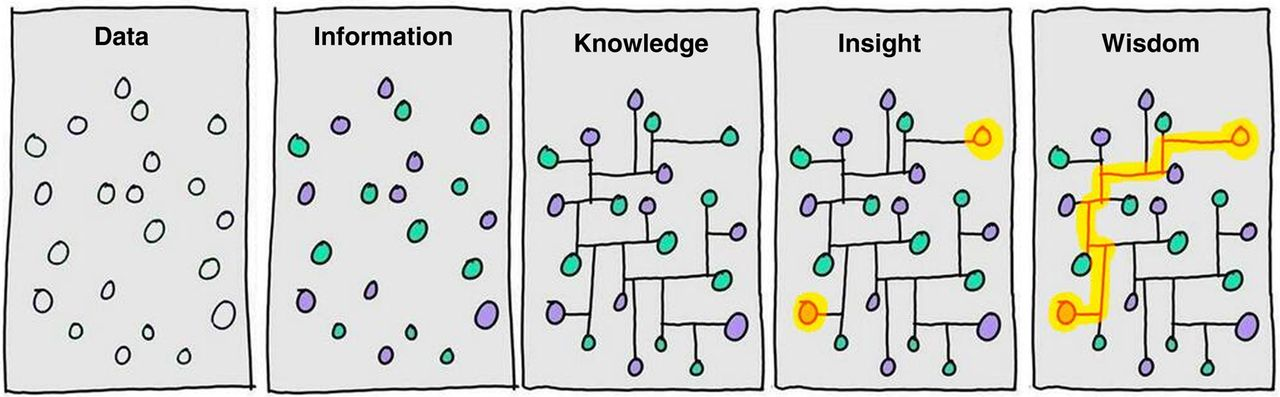
\includegraphics[width=0.8\linewidth]{figures-ext/01-Information_power} 

}

\caption{\textbf{From \emph{Data} to
\emph{Wisdom}}. Illustration of different steps that it takes to go from
\emph{Data} to generating \emph{Wisdom}. It highlights that generating
data is not equal to understanding it and additional efforts are needed
to generate value. Image authored by Clifford Stoll and Gary Schubert
published by Portland Press Limited on behalf of the Biochemical Society
and the Royal Society of Biology and distributed under the
\href{https://creativecommons.org/licenses/by/4.0/}{Creative Commons
Attribution License 4.0 (CC-BY)} in (\citet{BIG}
DATAOMICShttp://www.emergtoplifesci.org/content/1/3/245.article-info).}\label{fig:information-power}
\end{figure}












We will introduce most relevant data types that are used to study immune
infiltration of tumors.

\hypertarget{facs}{%
\subsection{Facs}\label{facs}}

\begin{quote}
Flow cytometry : Laser-based technology that allows for simultaneous
quantification of the abundance of up to 17 cell surface proteins using
fluorescently labelled antibodies. (\citet{Single-cell} RNA sequencing
to explore immune cell heterogeneity) cost : 0.05\$/ cell
\end{quote}

\begin{quote}
Mass cytometry(commercial name CyTOF). Mass spectrometry technique used
as an alternative to flow cytometry that allows for the quantification
of cellular protein levels by using isotopes that overcome problems
associated with the spectral overlap of fluorophores. 40 prot per cell
(\citet{Single-cell} RNA sequencing to explore immune cell
heterogeneity) 35\$/cell
\end{quote}

\hypertarget{staining}{%
\subsection{staining (histopathology, immunoscore!!! , multiplex
immunofluorescence)}\label{staining}}

\begin{quote}
The standardized Immunoscore was based on the quantification (cells/mm2)
of two lymphocyte populations (CD3 and CD8) within the central region
and the invasive margin of colorectal carcinoma tumors and provides a
scoring system ranging from Immunoscore 0 (I0) to Immunoscore 4 (I4)
(Figure 4).41 (\citet{Implications} of the tumor immune microenvironment
for staging and therapeutics Janis M Taube1,2,3, Jérôme Galon)
\end{quote}

\begin{quote}
The immune cell content of a tumour sample can also be determined by
using more established multiplexed methods like immunohistochemistry
(IHC) or immunofluorescence (IF)20 or newer methods like imaging mass
cytometry using FFPE tissue samples21. The advantage of these techniques
is that a larger number of cells can be analysed and that these
techniques also provide information about the spatial distribution of
the different cell types. However, these methods are limited to the
number of proteins that can be analysed simultaneously currently
(ranging from \textasciitilde{}10 to 100), advantage of the
deconvolution approach is that it is unbiased (i.e., hypothetical
response markers do not need to be pre-specified). It allows one to link
both the cellular characteristics and the cellular content with
treatment response. We anticipate that this approach will aid in the
discovery of novel predictive response biomarkers for both conventional
and immune-directed therapy by taking cellular composition into account.
(\citet{Shelker} et al.~Estimation of immune cell content using single
cell data).
\end{quote}

\hypertarget{omics}{%
\subsection{omics}\label{omics}}

Some kind of sequencing explanation needed for non-biologists

\hypertarget{transcriptome}{%
\subsubsection{transcriptome}\label{transcriptome}}

\begin{quote}
Bulk RNA-seq data can easily be obtained from either flash-frozen or
formalin-fixed, paraffin-embedded (FFPE) tissue samples, including both
surgically resected material and core needle biopsies. (\citet{Shelker}
et al.~Estimation of immune cell content using single cell data).
\end{quote}

\hypertarget{methylome}{%
\subsubsection{methylome}\label{methylome}}

\begin{quote}
Changes in gene expression in tumours owing to epigenetic modifi-cations
and the expression of microRNAs probably contribute directly to
determining the immune microenvironment and immunogenicity of a tumour.
Cytokine expression during T-cell development is regu-lated by
epigenetic alterations to both DNA and chromatin96. Cancer can also be
accompanied by epigenetic changes, which makes it prob-able that such
changes will influence cytokine profiles that modulate the immune
microenvironment. In fact, DNA methylation in lung-cancer cells has been
shown to reduce the expression of IL-1β97. And PD-L1 expression can be
modulated by microRNAs, with miR-200 (a repressor of
epithelial-to-mesenchymal transition) and possibly others decreasing its
expression98. Methylation of the promoter for the gene PD-L1 itself also
seems to repress PD-L1 expression; demethylation can result in
constitutive expression in tumours, especially non-small cell lung
cancer99..

Another influence on the immune profile of a tumour that has an
epigenetic mechanism involves the tissue of origin of the tumour.
Colorectal cancer tumours commonly express elevated levels of
transforming growth factor (TGF)-β100. Presumably, this reflects the
importance of the TGF-β pathway in intestinal biology and, especially,
its role in maintaining tolerance to the gut microbiota by favour-ing
the development of regulatory T~cells101. Elevated expression of TGF-β
may also contribute to the development of abundant stromal elements in
these tumours that can restrict the access of immune cells to the tumour
parenchyma, as has been demonstrated in pancreatic cancer102. Although
other factors also contribute, it is interesting to note that pancreatic
cancer and most forms of colorectal cancer (except for the mutationally
rich microsatellite-instability-high sub-group85) respond poorly to
single-agent inhibition of PD-L1/PD-1 (refs~62, 83 and~103--105).

(\citet{IMMUNE} CANCER CIRCLE)
\end{quote}

\hypertarget{single-cell}{%
\subsubsection{single cell}\label{single-cell}}

Described above methods of process DNA from hundreds of thousands of
cells simultaneously and report averaged gene expression of all cells.
In contrast, scRNA-seq technology allows getting results for each cell
individually. This is tremendous step forward enhancement of our
understanding of cell heterogeneity and opens new avenues of research
questions.

Continuous discovery of new immune subtypes has proven that cell surface
markers that are used for phenotyping by techniques like
\protect\hyperlink{facs}{FACS} and
\protect\hyperlink{staining}{immunohistochelistry} cannot capture the
full complexity. ScRNA-seq methods allow to cluster known cell types in
subpopulations based on their genetic features. (\citet{Single-cell} RNA
sequencing to explore immune cell heterogeneity). ScRNA-seq is also able
to capture particularly rare cell types as it requires much less of RNA
material (1 ng isolated from 100-1000 cells) compared to `bulk' RNA-seq
( \textasciitilde{} 1 μg of total mRNA transcripts )

\emph{new cellular states}

\begin{quote}
In summary, these studies have established that sur‑face phenotypes are
not sufficient to define cellular states in disease and have proposed
new scRNA‑seq methods to study innate immunological processes as well as
dis‑ease pathogenesis and progression at high resolution
(\citet{Single-cell} RNA sequencing to explore immune cell
heterogeneity)
\end{quote}

This new data type also brings into the field new challenges related to
data processing due to the volume, distribution, noise, and biases.
Experts highlight as the most ``problematic'' ``batch effect'' and noise
and ``dropout effect''
(\citet{https://www.nature.com/news/single-cell-sequencing-made-simple-1.22233}).
So far, there are no official standards that can be applied which makes
data comparison and post-processing even more challenging. Up to date,
there are around 70 reported tools and resources for single cell data
processing (@ GitHub, called `Awesome Single Cell'
(\href{http://go.nature.com/2rmb1hp}{go.nature.com/2rmb1hp})) .

A limited number of single-cell datasets of tumors are made publicly
available (\citet{TABLE}).

One can ask why then developing computational deconvolution of
transcriptome if we can learn relevant information from single-cell
data. Today's reality is that single cell data does not provide a
straightforward answer to the estimation of cell proportions. The
coverage is not full and sequenced single cells are not fully
representative of the true population. For instance, neutrophiles are
not found in scRNA-seq data because of they are ``difficult to isolate,
highly labile \emph{ex vivo} and therefore difficult to preserve with
current single-cell methods'' (\citet{Shelker} et al.~Estimation of
immune cell content using single cell data). In addition, a number of
patients included in published studies of range \textless{}100 cannot be
compared to thousand people cohorts sequenced with bulk transcriptome
methods. This is mostly because single cell experiments are challenging
to perform, especially in clinicsal setting as fresh samples are
needed.(\citet{Shelker} et al.~Estimation of immune cell content using
single cell data). Today, single cell technology brings very interesting
``zoom in'' perspective, but it would be incautious to make fundings
from a restricted group of individuals universal to the whole
population. Major brake to the use of single cell technology more
broadly might be as well the price that is neatly 10x higher for single
cell sample compared to bulk
(\citet{https://www.cedars-sinai.edu/Research/Research-Cores/Genomics-Core/Documents/Single-Cell-Genomics-Pricing}---June-2017.pdf).**
(A table? )**

\begin{longtable}[]{@{}cc@{}}
\toprule
Technology & Price per sample\tabularnewline
\midrule
\endhead
scRNA-seq & 3000 \$\tabularnewline
RNA-seq & 200 \$\tabularnewline
\bottomrule
\end{longtable}

In this work, we are using single cell data in two ways. Firstly, in
\protect\hyperlink{results}{Comparative\ldots{} chapter} we compare
immune cell profiles defined by scRNA-seq, blood and blind deconvolution
(problem introduced in \protect\hyperlink{immune-signatures}{Immune
signatures section}). Secondly, in \protect\hyperlink{map}{Heterogeneity
of immune\ldots{}} we use single call data of Metastatic melanoma
generated by Tirosh et al. (\citet{Tirosh} Melanoma sc) to demonstrate
subpopulations of Macrophages and NK cells.

\hypertarget{methods}{%
\chapter{Mathematical foundation of deconvolution}\label{methods}}

Here is a review of existing methods.

\hypertarget{deconvolution-of-transcriptomes-and-methylomes}{%
\chapter{Deconvolution of transcriptomes and
methylomes}\label{deconvolution-of-transcriptomes-and-methylomes}}

We describe our methods in this chapter.

\hypertarget{results}{%
\chapter{Comparative analysis of cancer immune
infiltration}\label{results}}

Some \emph{significant} applications are demonstrated in this chapter.

\hypertarget{example-one}{%
\section{Example one}\label{example-one}}

\hypertarget{example-two}{%
\section{Example two}\label{example-two}}

\hypertarget{map}{%
\chapter{Heterogeneity of immune cell types}\label{map}}

We have finished a nice book.

\hypertarget{annexes}{%
\chapter*{Annexes}\label{annexes}}
\addcontentsline{toc}{chapter}{Annexes}

\bibliography{book.bib,packages.bib}


\end{document}
